\documentclass[11pt]{article}
\usepackage{amsmath}
\usepackage{amssymb}
\usepackage{graphicx}
\usepackage{tabularx}
\usepackage{fancyhdr}
\usepackage{lastpage}

% Page layout
\usepackage[top=1in, bottom=1in, left=1in, right=1in]{geometry}

% Header and footer
\pagestyle{fancy}
\fancyhf{}
\rfoot{Page \thepage}
\renewcommand{\headrulewidth}{0pt}

% Modified Question command with left-aligned number
\newcommand{\questiona}[2]{
    \noindent\textbf{Q#2.} #1 \hfill \textbf{[1 Mark]}
}

\newcommand{\questionb}[2]{
    \noindent\textbf{Q#2.} #1 \hfill \textbf{[2 Marks]}
}

\begin{document}

% Title section with horizontal line
\begin{center}
    \Large\textbf{GATE 2018 - Biotechnology (BT)} \\
    \large\textbf{General Aptitude and Technical Questions} \\
    \rule{\textwidth}{0.5pt} % Horizontal line below heading
\end{center}

\vspace{0.5cm}

% General Aptitude Section
\section*{General Aptitude}

\questiona{"When she fell down the \_\_\_\_\_, she received many \_\_\_\_\_ but little help." The words that best fill the blanks in the above sentence are}{1}
\begin{enumerate}
    \item[(A)] stairs, stares  
    \item[(B)] stairs, stairs  
    \item[(C)] stares, stairs  
    \item[(D)] stares, stares  
\end{enumerate}
\vspace{0.5cm}

\questiona{"In spite of being warned repeatedly, he failed to correct his \_\_\_\_\_ behaviour." The word that best fills the blank in the above sentence is}{2}
\begin{enumerate}
    \item[(A)] rational  
    \item[(B)] reasonable  
    \item[(C)] errant  
    \item[(D)] good  
\end{enumerate}
\vspace{0.5cm}

\questiona{For \(0 \leq x \leq 2\pi\), \(\sin x\) and \(\cos x\) are both decreasing functions in the interval \_\_\_\_\_.}{3}
\begin{enumerate}
    \item[(A)] \(\left(0, \frac{\pi}{2}\right)\)  
    \item[(B)] \(\left(\frac{\pi}{2}, \pi\right)\)  
    \item[(C)] \(\left(\pi, \frac{3\pi}{2}\right)\)  
    \item[(D)] \(\left(\frac{3\pi}{2}, 2\pi\right)\)  
\end{enumerate}
\vspace{0.5cm}

\questiona{The area of an equilateral triangle is \(\sqrt{3}\). What is the perimeter of the triangle?}{4}
\begin{enumerate}
    \item[(A)] 2  
    \item[(B)] 4  
    \item[(C)] 6  
    \item[(D)] 8  
\end{enumerate}
\vspace{0.5cm}

\questiona{Arrange the following three-dimensional objects in the descending order of their volumes:
\begin{enumerate}
    \item A cuboid with dimensions 10 cm, 8 cm and 6 cm
    \item A cube of side 8 cm
    \item A cylinder with base radius 7 cm and height 7 cm
    \item A sphere of radius 7 cm
\end{enumerate}}{5}
\begin{enumerate}
    \item[(A)] (i), (ii), (iii), (iv)  
    \item[(B)] (ii), (i), (iv), (iii)  
    \item[(C)] (iii), (ii), (i), (iv)  
    \item[(D)] (iv), (iii), (ii), (i)  
\end{enumerate}
\vspace{0.5cm}

\questionb{An automobile travels from city A to city B and returns to city A by the same route. The speed of the vehicle during the onward and return journeys were constant at 60 km/h and 90 km/h, respectively. What is the average speed in km/h for the entire journey?}{6}
\begin{enumerate}
    \item[(A)] 72  
    \item[(B)] 73  
    \item[(C)] 74  
    \item[(D)] 75  
\end{enumerate}
\vspace{0.5cm}

\questionb{A set of 4 parallel lines intersect with another set of 5 parallel lines. How many parallelograms are formed?}{7}
\begin{enumerate}
    \item[(A)] 20  
    \item[(B)] 48  
    \item[(C)] 60  
    \item[(D)] 72  
\end{enumerate}
\vspace{0.5cm}

\questionb{To pass a test, a candidate needs to answer at least 2 out of 3 questions correctly. A total of 6,30,000 candidates appeared for the test. Question A was correctly answered by 3,30,000 candidates. Question B was answered correctly by 2,50,000 candidates. Question C was answered correctly by 2,60,000 candidates. Both questions A and B were answered correctly by 1,00,000 candidates. Both questions B and C were answered correctly by 90,000 candidates. Both questions A and C were answered correctly by 80,000 candidates. If the number of students answering all questions correctly is the same as the number answering none, how many candidates failed to clear the test?}{8}
\begin{enumerate}
    \item[(A)] 30,000  
    \item[(B)] 2,70,000  
    \item[(C)] 3,90,000  
    \item[(D)] 4,20,000  
\end{enumerate}
\vspace{0.5cm}

\questionb{If \(x^2 + x - 1 = 0\) what is the value of \(x^4 + \frac{1}{x^4}\)?}{9}
\begin{enumerate}
    \item[(A)] 1  
    \item[(B)] 5  
    \item[(C)] 7  
    \item[(D)] 9  
\end{enumerate}
\vspace{0.5cm}

\questionb{In a detailed study of annual crow births in India, it was found that there was relatively no growth during the period 2002 to 2004 and a sudden spike from 2004 to 2005. In another unrelated study, it was found that the revenue from cracker sales in India which remained fairly flat from 2002 to 2004, saw a sudden spike in 2005 before declining again in 2006. The solid line in the graph below refers to annual sale of crackers and the dashed line refers to the annual crow births in India. Choose the most appropriate inference from the above data.}{10}
\begin{center}
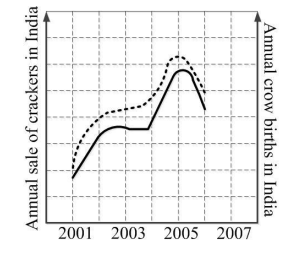
\includegraphics[width=0.5\textwidth]{figures/10.png}
\end{center}
\begin{enumerate}
    \item[(A)] There is a strong correlation between crow birth and cracker sales.  
    \item[(B)] Cracker usage increases crow birth rate.  
    \item[(C)] If cracker sale declines, crow birth will decline.  
    \item[(D)] Increased birth rate of crows will cause an increase in the sale of crackers.  
\end{enumerate}
\vspace{0.5cm}

% Technical Section
\section*{Technical Section}

\questiona{Consider an unfair coin. The probability of getting heads is 0.6. If you toss this coin twice, what is the probability that the first or the second toss is heads?}{1}
\begin{enumerate}
    \item[(A)] 0.56  
    \item[(B)] 0.64  
    \item[(C)] 0.84  
    \item[(D)] 0.96  
\end{enumerate}
\vspace{0.5cm}

\questiona{If serum is removed from the growth medium of human embryonic kidney cell line (HEK), then the cells will}{2}
\begin{enumerate}
    \item[(A)] proliferate faster  
    \item[(B)] proliferate normally  
    \item[(C)] undergo cell cycle arrest  
    \item[(D)] undergo immediate apoptosis  
\end{enumerate}
\vspace{0.5cm}

\questiona{The repeat sequence of telomere in humans is}{3}
\begin{enumerate}
    \item[(A)] 5-TATAAT-3 
    \item[(B)] 5-TTAGGG-3
    \item[(C)] 5-GGGCCC-3  
    \item[(D)] 5-AAAAAA-3
\end{enumerate}
\vspace{0.5cm}

\questiona{If a segment of a sense strand of DNA is 5-ATGGACCAGA-3, then the resulting RNA sequence after transcription is}{4}
\begin{enumerate}
    \item[(A)] 5-AGACCAGGTA-3  
    \item[(B)] 5-UCUGGUCCAU-3  
    \item[(C)] 5-UACCUGGUCU-3  
    \item[(D)] 5-AUGGACCAGA-3 
\end{enumerate}
\vspace{0.5cm}

\questiona{Which one of the following is an example of a neurotoxin?}{5}
\begin{enumerate}
    \item[(A)] Cholera toxin  
    \item[(B)] Streptolysin-O  
    \item[(C)] Botulinum toxin  
    \item[(D)] Diphtheria toxin  
\end{enumerate}
\vspace{0.5cm}

\questiona{Which of the following components constitute a molecular mechanics force field?}{6}
\begin{enumerate}
    \item[P.] Bond stretching  
    \item[Q.] Bond angle bending  
    \item[R.] Torsional bond rotation  
    \item[S.] Non-bonded interactions  
    \item[(A)] P and Q only  
    \item[(B)] P, Q and R only  
    \item[(C)] P, Q and S only  
    \item[(D)] P, Q, R and S  
\end{enumerate}
\vspace{0.5cm}

\questiona{Which one of the following BLAST search programs is used to identify homologs of a genomic DNA query in a protein sequence database?}{7}
\begin{enumerate}
    \item[(A)] blastp  
    \item[(B)] blastn  
    \item[(C)] blastx  
    \item[(D)] tblastn  
\end{enumerate}
\vspace{0.5cm}

\questiona{A mixture contains three similarly sized peptides P, Q and R. The peptide P is positively charged, Q is weakly negative and R is strongly negative. If this mixture is passed through an ion-exchange chromatography column containing an anionic resin, their order of elution will be}{8}
\begin{enumerate}
    \item[(A)] P, Q, R  
    \item[(B)] R, Q, P  
    \item[(C)] Q, R, P  
    \item[(D)] P, Q and R elute together  
\end{enumerate}
\vspace{0.5cm}

\questiona{Which one of the following is INCORRECT about protein structures?}{9}
\begin{enumerate}
    \item[(A)] A protein fold is stabilized by favorable non-covalent interactions  
    \item[(B)] All parts of a fold can be classified as helices, strands or turns  
    \item[(C)] Two non-covalent atoms cannot be closer than the sum of their van der Waals radii  
    \item[(D)] The peptide bond is nearly planar  
\end{enumerate}
\vspace{0.5cm}

\questiona{Which one of the following metabolic processes in mammalian cells does NOT occur in the mitochondria?}{10}
\begin{enumerate}
    \item[(A)] Citric acid cycle  
    \item[(B)] Oxidative phosphorylation  
    \item[(C)] Fatty acid $\beta$-oxidation  
    \item[(D)] Glycolysis  
\end{enumerate}
\vspace{0.5cm}

\questiona{Which one of the following is NOT a principal component of innate immunity?}{11}
\begin{enumerate}
    \item[(A)] Mucosal epithelia  
    \item[(B)] Dendritic cells  
    \item[(C)] Complement system  
    \item[(D)] Memory B-cells  
\end{enumerate}
\vspace{0.5cm}

\questiona{Which of the following technique(s) can be used to study conformational changes in myoglobin?}{12}
\begin{enumerate}
    \item[P.] Mass spectrometry  
    \item[Q.] Fluorescence spectroscopy  
    \item[R.] Circular dichroism spectroscopy  
    \item[S.] Light microscopy  
    \item[(A)] P only  
    \item[(B)] P and S only  
    \item[(C)] Q and R only  
    \item[(D)] S only  
\end{enumerate}
\vspace{0.5cm}

\questiona{Which one of the following bioreactor configurations is the basis for a trickling biological filter?}{13}
\begin{enumerate}
    \item[(A)] Stirred tank  
    \item[(B)] Packed bed  
    \item[(C)] Air lift  
    \item[(D)] Fluidized bed  
\end{enumerate}
\vspace{0.5cm}

\questiona{Cell type A secretes molecule X into the culture medium. Cell type B in the same culture responds to the molecule X by expressing protein Y. Which one of the following modes of signaling represents the interaction between A and B?}{14}
\begin{enumerate}
    \item[(A)] Autocrine  
    \item[(B)] Juxtacrine  
    \item[(C)] Paracrine  
    \item[(D)] Intracrine  
\end{enumerate}
\vspace{0.5cm}

\questiona{Which one of the following statements is true for actin?}{15}
\begin{enumerate}
    \item[(A)] Actin filament is structurally polarized and the two ends are not identical  
    \item[(B)] De novo actin polymerization is a single-step process  
    \item[(C)] The pointed end of the actin filaments is the fast growing end  
    \item[(D)] Actin forms spindle fibers during mitosis  
\end{enumerate}
\vspace{0.5cm}

\questiona{Standard error is}{16}
\begin{enumerate}
    \item[(A)] the probability of a type I error in a statistical test  
    \item[(B)] the error in estimating a sample standard deviation  
    \item[(C)] the standard deviation of a variable that follows standard normal distribution  
    \item[(D)] the standard deviation of distribution of sample means  
\end{enumerate}
\vspace{0.5cm}

\questiona{Which one of the following techniques is used to monitor RNA transcripts, both temporally and spatially?}{17}
\begin{enumerate}
    \item[(A)] Northern blotting  
    \item[(B)] In situ hybridization  
    \item[(C)] Southern blotting  
    \item[(D)] Western blotting  
\end{enumerate}
\vspace{0.5cm}

\questiona{Identify the character based method(s) used for the construction of a phylogenetic tree.}{18}
\begin{enumerate}
    \item[P.] Maximum parsimony  
    \item[Q.] Neighbor joining  
    \item[R.] Maximum likelihood  
    \item[S.] Bootstrapping  
    \item[(A)] Q only  
    \item[(B)] P and R only  
    \item[(C)] Q and S only  
    \item[(D)] S only  
\end{enumerate}
\vspace{0.5cm}

\questiona{Which one of the following is the solution for \( \cos^2 x + 2 \cos x + 1 = 0 \), for values of \( x \) in the range of \( 0^\circ < x < 360^\circ \)?}{19}
\begin{enumerate}
    \item[(A)] 45°  
    \item[(B)] 90°  
    \item[(C)] 180°  
    \item[(D)] 270°  
\end{enumerate}
\vspace{0.5cm}

\questiona{Which one of the following plant secondary metabolites is a natural insecticide?}{20}
\begin{enumerate}
    \item[(A)] Digitoxin  
    \item[(B)] Pyrethrin  
    \item[(C)] Salicylic acid  
    \item[(D)] Avenacin A-1  
\end{enumerate}
\vspace{0.5cm}

\questiona{The determinant of the matrix \(\begin{bmatrix} 4 & -6 \\ -3 & 2 \end{bmatrix}\) is}{21}
\vspace{0.5cm}

\questiona{The variable \( z \) has a standard normal distribution. If \( P(0 \leq z \leq 1) = 0.34 \), then \( P(z^2 > 1) \) is equal to (up to two decimal places)}{22}
\vspace{0.5cm}

\questiona{The absorbance of a solution of tryptophan measured at 280 nm in a cuvette of 2.0 cm path length is 0.56 at pH 7. The molar extinction coefficient (\( \epsilon \)) for tryptophan at 280 nm is 5600 M\(^{-1}\)cm\(^{-1}\) at pH 7. The concentration of tryptophan (in $\mu$M) in the solution is}{23}
\vspace{0.5cm}

\questiona{A single stem cell undergoes 10 asymmetric cell divisions. The number of stem cells at the end is}{24}
\vspace{0.5cm}

\questiona{Genomic DNA isolated from a bacterium was digested with a restriction enzyme that recognizes a 6-base pair (bp) sequence. Assuming random distribution of bases, the average length (in bp) of the fragments generated is}{25}
\vspace{0.5cm}

\questionb{In leguminous plants, both the rhizobium genes and the plant genes influence nodulation and nitrogen fixation. Which one of the following functions is NOT encoded by the host plant genes?}{26}
\begin{enumerate}
    \item[(A)] Production of inducers that modify rhizobial cell wall
    \item[(B)] Production of flavonoid inducers
    \item[(C)] Establishment of contact between bacteria and legume
    \item[(D)] Root hair curling
\end{enumerate}
\vspace{0.5cm}

\questionb{Which of the following cytokines are endogenous pyrogens?}{27}
\begin{enumerate}
    \item[P.] Tumor necrosis factor-$\alpha$
    \item[Q.] Interleukin-1
    \item[R.] Transforming growth factor-$\beta$
    \item[S.] Interleukin-10
    \item[(A)] P and Q only
    \item[(B)] P and R only
    \item[(C)] R and S only
    \item[(D)] Q and S only
\end{enumerate}
\vspace{0.5cm}

\questionb{Match the classes of RNA molecules in Group I with their functions in Group II.}{28}
\begin{tabular}{ll}
Group I & Group II \\
P. snqRNA & 1. Protects germline from transposable elements \\
Q. pjRNA & 2. Blocks translation of selected mRNA \\
R. miRNA & 3. Template for telomere elongation \\
S. snRNA & 4. Modification and processing of rRNA \\
 & 5. Splicing of RNA transcripts \\
\end{tabular}
\begin{enumerate}
    \item[(A)] P-3, Q-5, R-2, S-4
    \item[(B)] P-1, Q-3, R-2, S-5
    \item[(C)] P-1, Q-4, R-5, S-2
    \item[(D)] P-4, Q-1, R-2, S-5
\end{enumerate}
\vspace{0.5cm}

\questionb{Determine the correctness or otherwise of the following Assertion [a] and the Reason [r]}{29}
\textbf{Assertion:} Ab initio gene finding algorithms that predict protein coding genes in eukaryotic genomes are not completely accurate. \\
\textbf{Reason:} Eukaryotic splice sites are difficult to predict.
\begin{enumerate}
    \item[(A)] Both [a] and [r] are false
    \item[(B)] [a] is true but [r] is false
    \item[(C)] Both [a] and [r] are true and [r] is the correct reason for [a]
    \item[(D)] Both [a] and [r] are true but [r] is not the correct reason for [a]
\end{enumerate}
\vspace{0.5cm}

\questionb{Which one of the following amino acids is catalyzed by activated macrophages to produce reactive nitrogen species?}{30}
\begin{enumerate}
    \item[(A)] Arginine
    \item[(B)] Asparagine
    \item[(C)] Cysteine
    \item[(D)] Histidine
\end{enumerate}
\vspace{0.5cm}

\questionb{Determine the correctness or otherwise of the following Assertion [a] and the Reason [r]}{31}
\textbf{Assertion:} The association constant in water for the G-C base pair is three times lower than that for the A-T base pair. \\
\textbf{Reason:} There are three hydrogen bonds in the G-C base pair and two in the A-T base pair.
\begin{enumerate}
    \item[(A)] Both [a] and [r] are true and [r] is the correct reason for [a]
    \item[(B)] [a] is false but [r] is true
    \item[(C)] Both [a] and [r] are false
    \item[(D)] Both [a] and [r] are true and [r] is not the correct reason for [a]
\end{enumerate}
\vspace{0.5cm}

\questionb{Which one of the combinations of the following statements is true about antibody structure?}{32}
\begin{enumerate}
    \item[P.] Limited proteolysis of rabbit IgG with the enzyme pepsin generates two antigen-binding regions (Fab) and an Fc fragment
    \item[Q.] Limited proteolysis of rabbit IgG with the enzyme papain generates a single bivalent antigen-binding region $F(ab')_2$ and peptide fragments
    \item[R.] The Fc fragment of IgG can self-associate and crystallize into a lattice
    \item[S.] The $F(ab')_2$ fragment of IgG is composed of both light and heavy chains
    \item[(A)] P and Q only
    \item[(B)] P and R only
    \item[(C)] R and S only
    \item[(D)] Q and S only
\end{enumerate}
\vspace{0.5cm}

\questionb{Which one of the following statements is true with regard to processing and presentation of protein antigens?}{33}
\begin{enumerate}
    \item[(A)] In the class II MHC pathway, protein antigens in the cytosol are processed by proteasomes
    \item[(B)] In the class I MHC pathway, extracellular protein antigens are endocytosed into vesicles and processed
    \item[(C)] In the class I MHC pathway, transporter associated antigen processing (TAP) protein is required for translocating processed peptides generated in the cytosol
    \item[(D)] Invariant chain in endoplasmic reticulum is involved in transport of peptides and loading of class I MHC
\end{enumerate}
\vspace{0.5cm}

\questionb{Which of the following are true about bacterial superoxide dismutase?}{34}
\begin{enumerate}
    \item[P.] Present in obligate aerobes
    \item[Q.] Present in facultative anaerobes
    \item[R.] Present in aerotolerant anaerobes
    \item[S.] Absent in obligate aerobes
    \item[(A)] P and Q only
    \item[(B)] P, Q and R only
    \item[(C)] P and R only
    \item[(D)] Q and S only
\end{enumerate}
\vspace{0.5cm}

\questionb{Which of the following are true with regard to anaerobic respiration in bacteria?}{35}
\begin{enumerate}
    \item[P.] The final electron acceptor is an inorganic substance other than molecular oxygen
    \item[Q.] The number of ATP molecules produced per glucose molecule is more than that produced in aerobic respiration
    \item[R.] The number of ATP molecules produced per glucose molecule is less than that produced in aerobic respiration
    \item[S.] Only substrate level phosphorylation is used to generate ATP
    \item[(A)] P and S only
    \item[(B)] Q and S only
    \item[(C)] P and R only
    \item[(D)] P, Q and S only
\end{enumerate}
\vspace{0.5cm}

\questionb{Shear stress versus shear rate behavior of four different types of fluids (I, II, III and IV) are shown in the figure below.}{36}
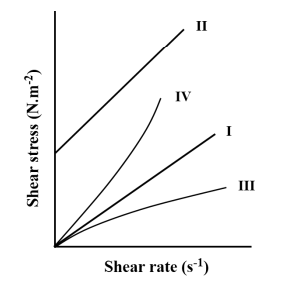
\includegraphics[width=0.5\textwidth]{figures/Q36}
Which one of the following options is correct?
\begin{enumerate}
    \item[(A)] I-Newtonian, II-Bingham plastic, III-Dilatant, IV-Pseudoplastic
    \item[(B)] I-Pseudoplastic, II-Dilatant, III-Newtonian, IV-Bingham plastic
    \item[(C)] I-Newtonian, II-Pseudoplastic, III-Bingham plastic, IV-Dilatant
    \item[(D)] I-Newtonian, II-Bingham plastic, III-Pseudoplastic, IV-Dilatant
\end{enumerate}
\vspace{0.5cm}

\questionb{An analysis of DNA-protein interactions was carried out using all DNA-protein complexes in the protein data bank (PDB). The frequency distribution of four amino acid residues, represented as P, Q, R and S, occurring in non-covalent interactions between the protein and DNA backbone is shown below.}{37}
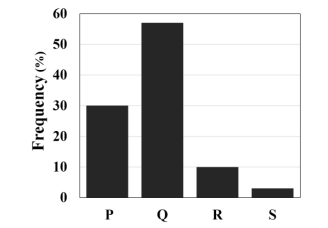
\includegraphics[width=0.5\textwidth]{figures/Q37}
Which one of the following is correct?
\begin{enumerate}
    \item[(A)] P-Lys, Q-Arg, R-Gln, S-Glu
    \item[(B)] P-Gln, Q-Glu, R-Lys, S-Arg
    \item[(C)] P-Asn, Q-Asp, R-Arg, S-Lys
    \item[(D)] P-His, Q-Glu, R-Gln, S-Lys
\end{enumerate}
\vspace{0.5cm}

\questionb{A pedigree of an inheritable disease is shown below.}{38}
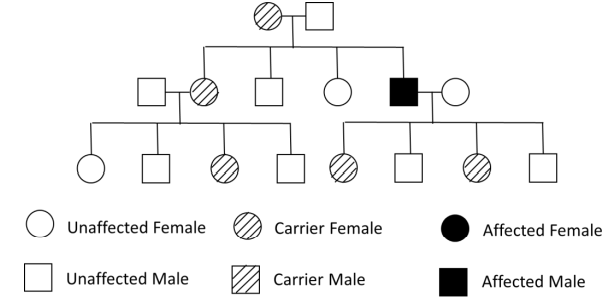
\includegraphics[width=0.5\textwidth]{figures/Q38}
What type of inheritance does the disease follow?
\begin{enumerate}
    \item[(A)] Autosomal dominant
    \item[(B)] X-linked dominant
    \item[(C)] X-linked recessive
    \item[(D)] Autosomal recessive
\end{enumerate}
\vspace{0.5cm}

\questionb{Match the industrial products mentioned in Group I with their producer organisms in Group II}{39}
\begin{tabular}{ll}
Group I & Group II \\
P. Citric acid & 1. Trichoderma viride \\
Q. Cellulase & 2. Clostridium acetobutylicum \\
R. Vitamin B12 & 3. Aspergillus niger \\
S. Butanol & 4. Propionibacterium freudenreichii \\
\end{tabular}
\begin{enumerate}
    \item[(A)] P-4, Q-3, R-1, S-2
    \item[(B)] P-3, Q-1, R-2, S-4
    \item[(C)] P-2, Q-1, R-4, S-3
    \item[(D)] P-3, Q-1, R-4, S-2
\end{enumerate}
\vspace{0.5cm}

\questionb{5' capping of mRNA transcripts in eukaryotes involves the following events:}{40}
\begin{enumerate}
    \item[P.] Addition of GMP on the 5' end
    \item[Q.] Removal of $\gamma$-phosphate of the triphosphate on first base at the 5' end
    \item[R.] 5'-5' linkage between GMP and the first base at 5' end
    \item[S.] Addition of methyl group to N7 position of guanine
\end{enumerate}
Which one of the following is the correct sequence of events?
\begin{enumerate}
    \item[(A)] P, Q, R, S
    \item[(B)] P, R, Q, S
    \item[(C)] Q, P, R, S
    \item[(D)] Q, P, S, R
\end{enumerate}
\vspace{0.5cm}

\questionb{Calculate the following integral (up to two decimal places)}{41}
\[ \int_0^1 (x + 3)(x + 1)dx = \]
\vspace{0.5cm}

\questionb{The probability distribution for a discrete random variable X is given below.}{42}
\begin{tabular}{|c|c|c|c|c|}
\hline
X & 1 & 2 & 3 & 4 \\
\hline
P(X) & 0.3 & 0.4 & 0.2 & 0.1 \\
\hline
\end{tabular}
The expectation value of X is (up to one decimal place)
\vspace{0.5cm}

\questionb{If \( 1 + r + r^2 + r^3 + \cdots \infty = 1.5 \), then, \( 1 + 2r + 3r^2 + 4r^3 + \cdots \infty = \) (up to two decimal places)}{43}
\vspace{0.5cm}

\questionb{Moist heat sterilization of spores at 121 °C follows first order kinetics as per the expression:}{44}
\[ \frac{dN}{dt} = -k_d N \]
where, \( N \) is the number of viable spores, \( t \) is the time, \( k_d \) is the rate constant and \( \frac{dN}{dt} \) is the rate of change of viable spores. \\
If \( k_d \) value is 1.0 min\(^{-1}\), the time (in minutes) required to reduce the number of viable spores from an initial value of 10\(^{10}\) to a final value of 1 is (up to two decimal places)
\vspace{0.5cm}

\questionb{An aqueous solution containing 6.8 mg/L of an antibiotic is extracted with amyl acetate. If the partition coefficient of the antibiotic is 170 and the ratio of water to solvent is 85, then the extraction factor is}{45}
\vspace{0.5cm}

\questionb{A microbial strain is cultured in a 100 L stirred fermenter for secondary metabolite production. If the specific rate of oxygen uptake is 0.4 h\(^{-1}\) and the oxygen solubility in the broth is 8 mg/L, then the volumetric mass transfer coefficient (\( K_{L}a \)) (in s\(^{-1}\)) of oxygen required to achieve a maximum cell concentration of 12 g/L is (up to two decimal places)}{46}
\vspace{0.5cm}

\questionb{In a chemostat, the feed flow rate and culture volume are 100 ml/h and 1.0 L, respectively. With glucose as substrate, the values of \(\mu_{max}\) and \(K_s\) are 0.2 h\(^{-1}\) and 1 g/L, respectively. For a glucose concentration of 10 g/L in the feed, the effluent substrate concentration (in g/L) is}{47}
\vspace{0.5cm}

\questionb{Mammalian cells in active growth phase were seeded at a density of 1×10\(^5\) cells/ml. After 72 hours, 1×10\(^6\) cells/ml were obtained. The population doubling time of the cells in hours is (up to two decimal places)}{48}
\vspace{0.5cm}

\questionb{Yeast converts glucose to ethanol and carbon dioxide by glycolysis as per the following reaction:}{49}
\[ C_6H_{12}O_6 \rightarrow 2C_2H_5OH + 2CO_2 \]
Assuming complete conversion, the amount of ethanol produced (in g) from 200 g of glucose is (up to two decimal places)
\vspace{0.5cm}

\questionb{At the end of a batch culture, glucose solution is added at a flow rate of 200 ml/h. If the culture volume after 2 h of glucose addition is 1000 ml, the initial culture volume (in ml) is}{50}
\vspace{0.5cm}

\questionb{Consider the following alignment of two DNA sequences:}{51}
\begin{verbatim}
AGTAAC
AA--AC
\end{verbatim}
Assuming an affine gap scoring scheme of an identity matrix for substitution, a gap initiation penalty of 1 and a gap extension penalty of 0.1, the score of the alignment is (up to one decimal place)
\vspace{0.5cm}

\questionb{First order deactivation rate constants for soluble and immobilized amyloglucosidase enzyme are 0.03 min\(^{-1}\) and 0.005 min\(^{-1}\), respectively. The ratio of half-life of the immobilized enzyme to that of the soluble enzyme is (rounded off to the nearest integer)}{52}
\vspace{0.5cm}

\questionb{Consider a simple uni-substrate enzyme that follows Michaelis-Menten kinetics. When the enzyme catalyzed reaction was carried out in the presence of 10 nM concentration of an inhibitor, there was no change in the maximal velocity. However, the slope of the Lineweaver-Burk plot increased 3-fold. The dissociation constant for the enzyme-inhibitor complex (in nM) is}{53}
\vspace{0.5cm}

\questionb{The product of complete digestion of the plasmid shown below with EcoRI and HaeIII was purified and used as a template in a reaction containing Klenow fragment of DNA polymerase, dNTPs and [$\alpha$-\(^{32}\)P]-dATP in a suitable reaction buffer. The product thus obtained was purified and subjected to gel electrophoresis followed by autoradiography.}{54}
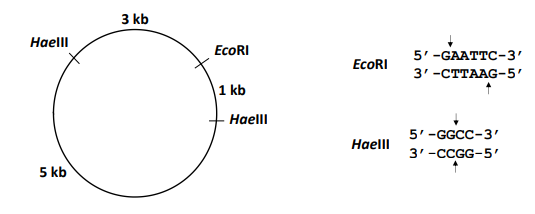
\includegraphics[width=0.5\textwidth]{figures/Q54}
The number of bands that will appear on the X-ray film is
\vspace{0.5cm}

\questionb{A rod shaped bacterium has a length of 2 µm, diameter of 1 µm and density the same as that of water. If proteins constitute 15\% of the cell mass and the average protein has a mass of 50 kDa, the number of proteins in the cell is}{55}
(1 Da = 1.6 × 10\(^{-24}\)g)
\vspace{1cm}

\begin{center}
\textbf{END OF THE QUESTION PAPER}
\rule{\textwidth}{0.5pt} 
\end{center}

\end{document}